\documentclass[conference,compsoc]{IEEEtran}
\usepackage{ifpdf}
\usepackage{caption}
\usepackage[pdftex]{graphicx}
\usepackage[noadjust]{cite}
\usepackage{amsmath}
\usepackage[caption=false,font=footnotesize,labelfont=sf,textfont=sf]{subfig}
\usepackage{fixltx2e}
\hyphenation{op-tical net-works semi-conduc-tor}
\renewcommand{\citedash}{--}


\begin{document}

\title{Visual Dataflow Language for Small Robots Programming}

\author{
	\IEEEauthorblockN{Grogorii Zimin}
	\IEEEauthorblockA{
		Mathematics and Mechanics Faculty,\\
		SPbSU\\
		Saint-Petersburg, Russia \\
		Email: zimin.grigory@gmail.com
	}
	
	\and

	\IEEEauthorblockN{Dmitrii Mordvinov}
	\IEEEauthorblockA{
		Mathematics and Mechanics Faculty,\\
		SPbSU\\
		Saint-Petersburg, Russia \\
		Email: mordvinov.dmitry@gmail.com
	}
}

\maketitle



\begin{abstract}
REWRITE THIS SH..
The paper describes dataflow visual programming language based on DSM-approach. Its purpose is to be bridge between lightweight robotics languages for education and complex industrial languages. A short review of programming languages for robots is presented here. Also different approaches and architectures for developing control system for robots are considered. For demonstration of language usage, the paper provide solution for creating control system of robot based on subsumption architecture. 
\end{abstract}

\section{Introduction}

Programming languages for creating robotic controllers are actual topics of research oftenly discussed at major conferences, such as ICRA\cite{Icra} or IROS\cite{Iros2016}. Visual programming languages (VPLs) are also actively discussed for the last three decades, the largest conferences are held annually, e.g. VL/HCC\cite{VLHCC}. VPLs are oftenly applied in robotics domain\cite{banyasad2000visual,simpson2006mobile,simpson2008visual,posso2011process,diprose2011ruru} allowing to create and visualize robotic controllers. Robotic VPLs are commonly used for educational purposes, making possible for students of even junior schools to create robotic programs. There already exists a great number of educational robotic programming environments based on VPLs, e.g. NXT-G\cite{nxtg}, TRIK Studio\cite{trik}, ROBOLAB\cite{robolab}, also there are some academic tools implementing interesting and novel approaches to educational robotics programming\cite{banyasad2000visual,simpson2008visual,diprose2011ruru}.

Robotic control programs have reactive nature: they transform data which is continuously coming from multiple sensors into the impulses on actuators. For this reason dataflow languages (DFLs) are well-suitable for robotics programming. Many researchers denoted the conveniency of dataflow visual programming languages (DFVPLs)\cite{johnston2004advances}, finding them more useful than textual DFLs, for example, because data flows explicitly displayed on the diagram. There are large and complex general-purpose and domain-specific development environments such as LabVIEW\cite{labview} and Simulink\cite{simulink} that provide a large (and sometimes even cumbersome) set of libraries for robotics programming. More detailed discussion of robotics VPLs will be provided in section~\ref{sec:Overview}.

There is a large number of robotic constructor kits for learning the basics of robotics and cybernetics, such as LEGO MINDSTORMS\cite{legokit}, TRIK, ScratchDuino\cite{http://www.scratchduino.com/}. Modern programming languages that are used for programming those kits are based on the control flow model rather than on dataflow model. Control flow-based languages are good for solving scholar "toy" tasks, but may be inconvenient for programming more complex "real world" controllers that may be conveniently expresses on DFLs. The simple DFVPL may be considered as a useful step from educational VPLs to the programming languages that are used in unversities and industry. 

In SPbSU cybernetic laboratory are conducted a number of studies aimed at improving the tools for design and programming of embedded systems for small robot platforms (e.g. LEGO, TRIK) using block diagrams\cite{}. Goal of research paper is the development of novel extensible tool for programming all small robot platforms which discussed above in dataflow style. While dataflow approach is commonly used approach when each element is executing in separate thread or process. Our approach avoids it, because it brings a large overhead on target platforms, details presented in section~\ref{sec:lang}. There are several commonly used robots controller architectures: Connell's Colony, Maes' Action-Selection, Arkin's Motor Schema, Rosenblatt's Distributed Architecture for Mobile Navigation, Brooks' Subsumption Architecture\cite{simpson2009toward}. DFLs are suitable for Brooks' Subsumption Architecture, his approach are commonly used\cite{banyasad2000visual,simpson2006mobile,posso2011process,proetzsch2007behaviour}. So, our approach also uses Brooks’ Subsumption Architecture as the fundamental concept used in the our DFVPL.

The paper is organized as follows. An overview of robotics VPL and DFVPL is presented in section~\ref{sec:Overview}. A description of our language are proposed in section~\ref{sec:lang}. Section~\ref{sec:robotControl} demonstrates typical robotic controller expressed in our language. Direction of future research works is given in section~\ref{sec:Future}. Finally, the last section concludes the paper.


\section{Overview and background}
\label{sec:Overview}
Robot programming environment can be divided into three categories: educational, which allows you to program small robots; industrial, which have a rich toolkit for creating robots control systems and different models; academic, which implement new interesting ideas, however, are often not available for download, or are not robust.

To educational, for example, can be referred EV3 Software development environment for the Lego Mindstorms EV3 kit, IDE NXT-G and ROBOLAB for LEGO MINDSTORMS NXT kit, TRIK kit and IDE TRIK Studio. These IDE make it easy to solve typical robot control tasks, e.g., find a way out of the maze, drive along the line using sensors by creation a primitive control system, which purpose is to teach the users the basics of programming and robot control. But their simplicity is bound with poor flexibility of the language. Actually these IDEs provide a consistent model of the robot control based on control flow model, that is described by visual graphical models.

In the industry there are very popular general-purpose IDE LabVIEW from National Instruments with the DFVPL G, and programming environment Simulink developed by MathWorks for modeling different dynamic models or control systems. These software products offer to the users a huge range of models and libraries to create any control systems, test benches, real-time systems, using model-driven approach. In particular, LabVIEW provides opportunity programming small robots. Although there is known of LabVIEW usage for educational purposes\cite{1_gomez-de-gabriel_mandow_fernandez-lozano_garcia-cerezo_2011}, most of the time in the educational process is spent on the study of the medium itself, not algorithms and robotic approaches. It should be noted that these environments are distributed under the commercial license.

Another example of an industrial system is the Microsoft Robotics Developer Studio (MSRDS)\cite{jackson2007microsoft}, which is free for academic use, and allow to easy create distributed robotic systems in terms of data flow, which components are represented as web services. MSRDS officially supports multiple robotic platforms, e.g., LEGO NXT\cite{kim2007programming}, for which, however, It does not support offline mode. MSRDS has the ability to integrate with  custom robotic platforms, but this environment is not supported in 2014.

There are a lot of research in this area, e.g., dissertation\cite{banyasad2000visual} describes a visual programming language in terms of extended machines Moore, \cite{simpson2008visual},\cite{posso2011process} describe visual $occam\mbox{-}\pi$ program editor and tools $Transterpreter$, and its usage in swarm robotics control system. Article\cite{diprose2011ruru} describes DFVPL for beginners and environment, which provides a comfortable interface. But the technology has too weak functionality and requires significant improvements, and doesn't available for download.

Based on the overview it is clear that no one of these environments is not suitable for programming small robots in terms of data flows. At the same time closest to the desirable is TRIK Studio, as it is the only medium, which distributed with open source with a highly scalable architecture, that has the ability to extend itself by new VPL for robots and provides opportunity to reuse code base of "routine" operations such as the interaction with the robot.



\section{DFVPL}
\label{sec:lang}
Evolution of a domain-specific modeling (DSM) methodology allows to quickly create a fairly sophisticated visual programming languages\cite{DSM}. TRIK Studio programming environment is an example of a system that was created using DSM-based approach on QReal platform\cite{qrealMeta, kuzenkova2013qreal}. Based on industrial experience of TRIK Studio developers, it had been decided to create the DFVPL based on QReal platform. We based our DFVPL on the several basic requirements.

\begin{itemize}
\item Brooks’ Subsumption Architecture should easily be expressed by means of language.
\item Robots behaviour diagram, as well as in TRIK Studio, should be have the opportunity to be interpreted on the two-dimensional simulation model of the robot or directly on robot via wi-fi.
\item Interpretation  of robots behaviour diagram  should emulate data flow common model, avoiding the strategy "one thread per block", but provides ability to manually create threads.
\end{itemize}


\subsection{Description of the blocks}
DFVPL block (element) is a entity which processes incoming on its channels data, and can emits result (or new data) on their output channels. Our DFVPL blocks can be divided into several groups.

\begin{itemize}
\item \textit{Control}. Blocks implementing design: conditions, loops, etc.
\begin{itemize}
\item \textit{Flow} implementing data transmission between others blocks (uses for connecting channels of blocks).
\item \textit{Fork, EndFork}. Blocks provide ability to force threading works.
\item \textit{RandomValue, ConstValue} Blocks are responsible for sending a random number or a predetermined value of any type.
\item \textit{GetSetVariable}. Pseudo DF block, which set value for given variable or emit it.
\item \textit{Loop, If, Switch}. These blocks implement common essence in DF style. \textit{Loop} is a custom entity which emitting the numbers or dummy data corresponding to predetermined settings. \textit{If} checks predetermined condition substituting variables by incoming data, and sends them to \textit{True} or \textit{False} channel. \textit{Switch} successively checks multiple conditions and if its evaluate as \textit{true} sends incoming data to corresponding channel.  	
\item \textit{Function} Block, which allows to make the processing of the input data in text language (PL Lua\cite{lua}), its support inherited from the code base of TRIK Studio). Most often, this block will be used for specifying mathematical operations on data.
\item \textit{FinalBlock} stops the execution of program, when receiving any data. 
\item \textit{SubprogramCall} is used to take out repetitive blocks on a separate diagram, and then use it as one block for data processing.
\item \textit{Wait} is simple block, which main goal is to delay data.
\item \textit{DelayFilter} is the evolution of the previous block, which add condition filtering and checking the number of emitted data validated by condition.
\end{itemize} 
\item \textit{Drawing}. Blocks for drawing on robots display and on the floor.
\begin{itemize}
\item \textit{Pen} is initialization block for drawing a predetermined color marker on the floor.  It controls the lowering and raising of the marker
\item \textit{PaintSettings} is block which used for define color of pen, background, width of the brush for drawing on robots display.
\item \textit{ShapePainter, SmilePainter, Text} are used for drawing some shape or text or smile on robots display. 
\item \textit{Clear} is block which clear robot display when receiving any data.
\end{itemize} 
\item \textit{Flow manipulation}. These elements provide opportunity to manipulate data which flow between blocks.
\begin{itemize}
\item \textit{InPort, OutPort}. Their purpose is the connecting incoming data to \textit{Subprogram} block and blocks which should received these data in it, and similarly from blocks in \textit{Subprogram} to output channels of \textit{Subprogram}. 
\item \textit{Supressor, Inhibitor} block or substitute data which flow via \textit{Flow}. These blocks and \textit{SubprogramCall} block provide support for the Brooks' Subsumption Architecture. 
\item \textit{Interflowing, Separator} provide opportunity to gather data from several \textit{Flows} into one and vice versa.
\end{itemize} 
\item \textit{Actions}. Blocks implements any actions which robot can make.
\begin{itemize}
\item \textit{Servo, Motors} process received data and send impulses to robot actuators.
\item \textit{Encoders} block sets the number of motor revolutions, when receiving data, and continuously emits current number for corresponding channels.
\item \textit{MessageToRobot, ReceiveMsg} responsible for the coordination of a group of robots. Sends data to specified robot via \textit{MessageToRobot}, and receive from any robots via \textit{ReceiveMsg}.
\item \textit{Say, PlayTone, Led} responsible for managing of sound and LED lights.
\item \textit{RemoveFile, WriteToFile} implement functions to working with files. \textit{WriteToFile} writes incoming data to specified file. \textit{RemoveFile} removes specified file or file which name it got from incoming data.
\item \textit{InitCamera, DetectByVideo, StreamingNode} provide access to all opportunities of video vision of TRIK controller: detect different objects and send data corresponding to specified (by incoming data or manually) object, stream video.
\item \textit{PortBlock} provides opportunities to write on some ports corresponding to robot device and emits data from it.
\item \textit{Sensor} continuously emits data from specified sensor, e.g. infrared, light, etc.
\item \textit{SystemCall} responsible for the command execution got from incoming data, e.g. "reboot" will reboot robot.
\item \textit{Gamepad} reads data from the control device, e.g. gamepad, and emits it.
\end{itemize} 
\end{itemize} 


One of the distinguishing features of our DFVPL is that some blocks are a single object on the diagram, and although it can be represented on the diagram in several places, only one of them works. It is modification of data flow paradigm which helps to work with our DFVPL as control flow VPL. For example figure~\ref{image:encoder} shows diagram with \textit{Motors, ConstValue, Encoders, Flows} where \textit{Encoders} block is presented twice. 

\begin{figure}[ht]
	\centering
	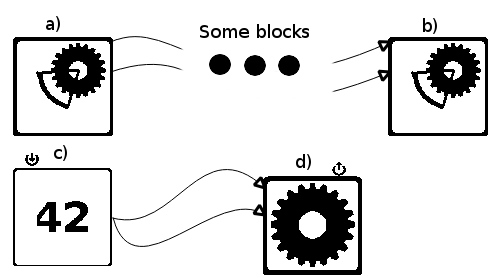
\includegraphics[width=3.5in]{Encoders.png}
	\caption{Block with many representations but only one of them can be active. a,b --- \textit{Encoders} c --- \textit{ConstValue} d --- \textit{Motors}}
	\label{image:encoder}
\end{figure}

When interpretation started \textit{ConstValue} emits data to \textit{Motors} and \textit{Encoders} (a) emits number of motor revolutions. After "Some blocks" \textit{Encoders} (b) receiving some data, which reinitialized block, at that moment \textit{Encoders} (a) stop emitting data (implementation details discussed in section~\ref{sec:impl}).

Let's describe some basic thing about our blocks. On figure~\ref{image:encoder} \textit{ConstValue} and \textit{Motors} have incoming and outgoing "arrows" to block, which are used to connect control flow data, e.g. \textit{Motors} emits data to control flow channel when handle incoming data, and \textit{ConstValue} emits its value when receive control flow data. On left, right and bottom side may be placed incoming and outgoing channels (points where \textit{Flows} may be pinned), which are signed when user edits block (see Figure~\ref{image:block}).
\begin{figure}[ht]
	\centering
	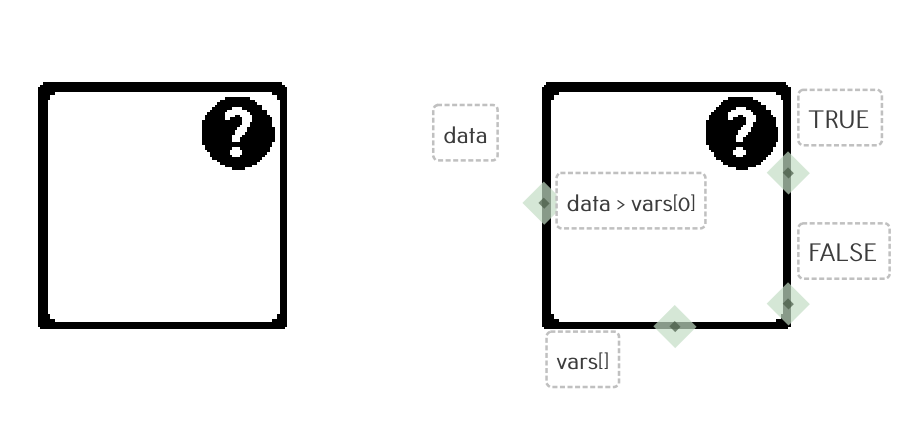
\includegraphics[width=3.5in]{block.png}
	\caption{Showing and editing of block.}
	\label{image:block}
\end{figure}
Also block may contain field for text, e.g. on Figure~\ref{image:block} user wrote condition.



These blocks are enough to control the robot and create varying complexity robot controllers, e.g. Figures~\ref{image:boxC},~\ref{image:box} show simple robot controller which control moving around box. Here we initialize some variables and regulate motors power based on the data continuously received from the infrared sensor. More complex, but typical robotic controller presented in section~\ref{sec:robotControl}. 

\begin{figure}[ht]
	\centering
	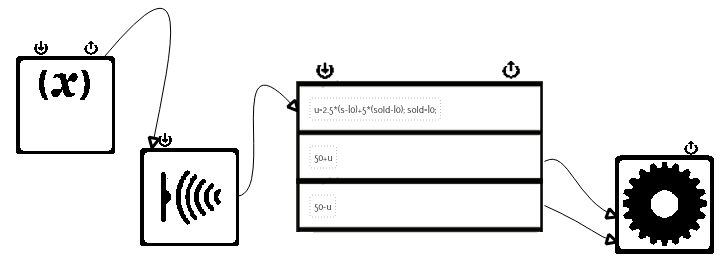
\includegraphics[width=3.5in]{alongBoxCode.png}
	\caption{Controller code for along box moving.}
	\label{image:boxC}
\end{figure}

\begin{figure}[ht]
	\centering
	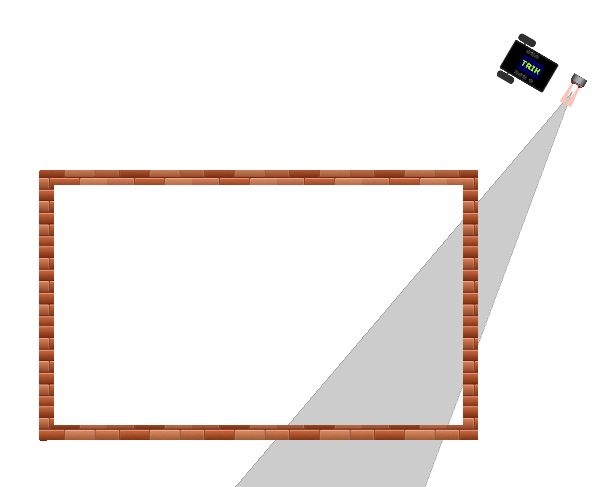
\includegraphics[width=3.5in]{alongBoxModel.png}
	\caption{Modelling of along box moving.}
	\label{image:box}
\end{figure}



\subsection{Pseudo dataflow}
The main direction of our language and programming tool is the small robots programming, so it was necessary to avoid the use of commonly used dataflow paradigm, when for each execution block created new thread or process. This method is perfect for larger and more complex robots equipped with powerful multi-core controllers. But for small robots linear increase in the number of blocks in the diagram will eventually reduce performance due to the overhead of thread- or process-switching.

So, our dataflow idiom was implemented as pseudo parallelism (see details in section~\ref{sec:impl}). But it is also exist opportunity to manually manage threads with two blocks --- \textit{Fork, EndFork}.

\section{Implementation details}	
\label{sec:impl}

\section{Robot control system}	
\label{sec:robotControl}
%Рассмотрим задачу управления движением робота при помощи джойстика, при условии, что робот сам избегает лобовых столкновений с припятствиями. Предполагается, что программа пишется для двухколесного мобильного робота, оборудованного спереди инфракрасными датчиками расстояния, для управления колесами используются силовые моторы.

%Разобьем задачу на два уровня поведения. Первый будет отвечать за обслуживание запросов пользователя. Второй будет ответственен за избегание столкновений: если робот близок к столкновению, то он должен уклониться от препятствия вне зависимости от того, что нажимает пользователь на пульте. 

%Рассмотрим первый уровень (рис.~\ref{image:layer1}). Пользователь управляет роботом посредством джойстика. Джойстик генерирует данные, соответствующие нажатиям кнопок или манипулирований рычагом направления. Для простоты считаем, что нажатие любой кнопки завершит программу управления роботом. Данные с рычага преобразуются блоком текстового программирования в соответствующие импульсы моторов робота, которые в данном случае передаются <<заглушкам>>, которые связаны с выходными портами блока <<Подпрограмма>>. 
%\begin{figure}[ht]
%	\centering
%	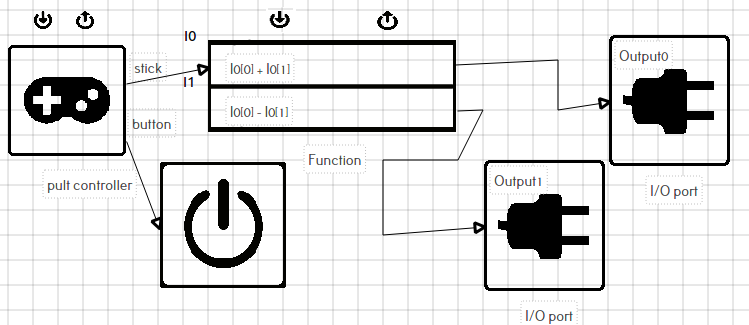
\includegraphics[width=3.5in]{pultLayer.png}
%	\caption{Уровень управления с пульта.}
%	\label{image:layer1}
%\end{figure}

%Рассмотрим второй уровень (рис.~\ref{image:layer2}): данные с датчиков расстояния собираются в вектор и передаются фильтру, который при опасности столкновения отправляет данные дальше в блок математической обработки (если условие не выполнилось, управление может быть передано по потоку <<ошибки>>, в данной программе этот поток не указан; также между проверками условия приходящие данные не обрабатываются (теряются) в течение установленного пользователем времени). В блоке математической обработки вычисляется мощность, которую необходимо подать на 2 мотора. Вычисленные значения передаются выходным портам.
%\begin{figure}[ht]
%	\centering
%	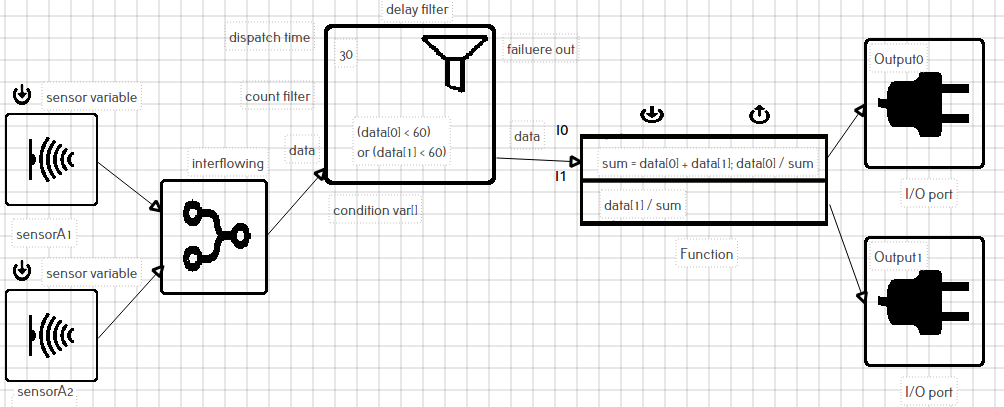
\includegraphics[width=3.5in]{collisionLayer.png}
%	\caption{Уровень избегания столкновений.}
%	\label{image:layer2}
%\end{figure}

%\begin{figure}[ht]
%	\centering
%	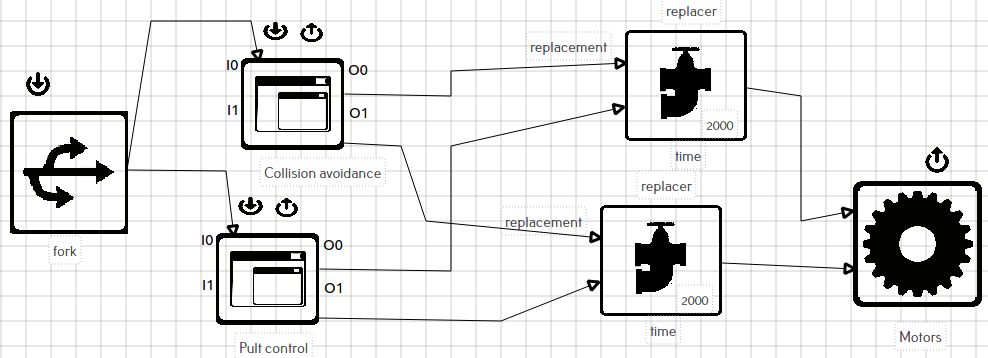
\includegraphics[width=3.5in]{programScreen.png}
%	\caption{Программа управления роботом.}
%	\label{image:prog}
%\end{figure}

%Имея два поведения, создаем управление роботом в модели Брукса (рис.~\ref{image:prog}). С помощью блока распараллеливания запускаем уровни поведения. Каждый уровень генерирует данные, соответствующие мощностям моторов, передаваемые на блок управления силовыми моторами. Так как второй уровень ответственности должен не позволить столкнуться с препятствием, его значения подавляют значения, полученные с первого уровня, с помощью блоков <<Подавления>>.

\section{Future works}
\label{sec:Future}

\section{Conclusion}
%На момент написания статьи был реализован прототип технологии програмирования роботов TRIK в терминах потоков данных. Система предоставляет возможность интерпретации диаграмм на двумерной имитационной модели робота и (в ближайшем будущем) генерации кода из диаграмм в текстовые языки, используемые для программирования TRIK (JavaScript, F\# и Kotlin). Также технология предоставляет поддержку архитектуры Брукса на уровне языка, что продемонстрировано в статье на примере операторского управления роботом с автоматическим избеганием столковений.

%Полученная система может рассматриваться как платформа для дальнейших научных исследований. К примеру, интересной представляется автоматическая генерации метамодели языка по спецификациям ПО промежуточного уровня на роботе (к примеру, ROS\footnote{http://www.ros.org/ [Дата обращения: 10 марта 2016]}). Другим направлением возможной работы является описание строгой семантики языка для применения различных формальных методов анализа программ, выраженных в нем.

\newpage
\bibliography{IEEEbibl}
\bibliographystyle{IEEEtran}
\end{document}
